\ylDisplay{Katus} % Ülesande nimi
{Jaan Kalda} % Autor
{lõppvoor} % Voor
{2017} % Aasta
{G 9} % Ülesande nr.
{9} % Raskustase
{
% Teema: Staatika
\ifStatement
Kaks jäika traadijuppi pikkusega $L$ on ühendatud otsapidi (nt niidiga seotud) nii, et nende otspunktid on kontaktis ja nende vaheline nurk saab takistuseta muutuda, moodustades V-kujulise figuuri. See traadist moodustis asetatakse horisontaalse libedapinnalise silindri peale nõnda, et tasakaaluasendis moodustub traadist \enquote{katus} (tagurpidi \enquote{V}) tipunurgaga $\alpha$. Massijaotus traadis on ühtlane, hõõre traadi ja silindri vahel puudub. a) Milline on silindri raadius $R$? b) Milline võrratus peab olema rahuldatud, et see asend oleks stabiilne (uurida stabiilsust vaid \enquote{katuse} kui terviku pöördumise suhtes, eeldades et traatidevaheline nurk ei muutu)?
\fi


\ifHint
Traadile mõjuvad kolm jõudu: raskusjõud ja traatide kontaktpunktis ning traadi ja silindri puutepunktis mõjuvad rõhumisjõud. Selleks, et traat tasakaalus oleks, peavad nende jõudude pikendused lõikuma ühes punktis (vastasel korral mõjuks kahe jõu lõikumispunkti suhtes kolmas jõud traadile nullist erineva jõumomendiga ja traat hakkaks liikuma).\\
Stabiilsuse analüüsis saab tähele panna, et kui \enquote{katus} pöörleb tervikuna, siis selle massikese liigub mööda ringjoont.
\fi


\ifSolution
Kahe traadi kontaktpunktis $A$ (vaata joonist allpool) mõjutavad traadid sümmeetria ja Newtoni III seaduse tõttu üksteist 
horisontaalsete vastassuunaliste jõududega; traadi ja silindri puutepunktis $B$ mõjub traadile rõhumisjõud, mis on traadiga risti ning seetõttu läbib selle jõu pikendus silindri telge $Q$. Raskusjõud on rakendatud traadi keskpunkti $C$. Et traat on tasakaalus ja talle mõjuvad kolmes punktis jõud, siis nende jõudude pikendused peavad lõikuma ühes punktis $O$ (vastasel korral mõjuks kahe jõu lõikumispunkti suhtes kolmas jõud traadile nullist erineva jõumomendiga ja traat hakkaks liikuma). Niisiis peavad punktist $A$ tõmmatud horisontaal, punktist $C$ tõmmatud vertikaal ning sirge $QB$ pikendus kõik lõikuma ühes punktis. Paneme tähele, et $\angle ACO=\alpha/2$ ja $\angle AOB=\alpha/2$, seetõttu
$$|AO|=|AC|\sin(\alpha/2)=(L/2)\sin(\alpha/2),$$ $$|AB|=|AO|\sin(\alpha/2)=(L/2)\sin^2(\alpha/2)$$ ning
$$R=|QB|=|AB|\tan(\alpha/2)=(L/2)\sin^3(\alpha/2)/\cos(\alpha/2).$$

\begin{center}
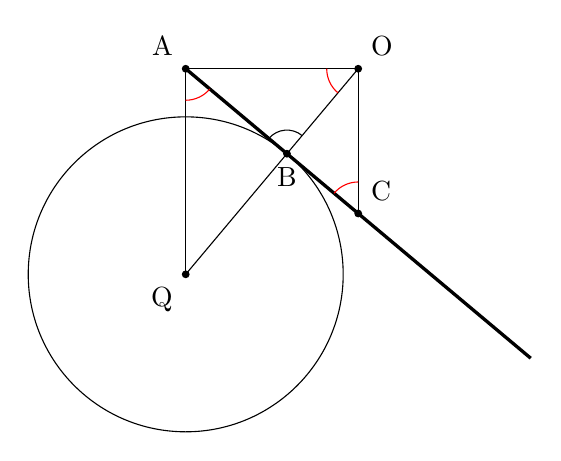
\begin{tikzpicture}
\usetikzlibrary{calc}
\def\angKatus{50};
\def\rKatus{2};
\coordinate (P1) at (0,{\rKatus/sin(\angKatus)});
\coordinate (P2) at ({\rKatus/sin(\angKatus)/tan(\angKatus)},{\rKatus/sin(\angKatus)});
\coordinate (P3) at ({\rKatus/sin(\angKatus)/tan(\angKatus)},{\rKatus/sin(\angKatus)-\rKatus/sin(\angKatus)/tan(\angKatus)/tan(\angKatus)});
%\fill (0,0) circle (0.05);
\node [label=below left:Q, fill=black, circle,inner sep=1pt] at (0,0){};
\draw (0,0) circle (\rKatus);
\node [label=above left:A, fill=black, circle,inner sep=1pt] at (P1){};
\node [label=above right:O, fill=black, circle,inner sep=1pt] at (P2){};
\node [label=above right:C, fill=black, circle,inner sep=1pt] at (P3){};
\node [label=below:B, fill=black, circle,inner sep=1pt] at (\angKatus:\rKatus){};
\draw [very thick](P1) -- (P3) -- ++($(P3)-(P1)$);
\draw (0,0) -- (P2);
\draw (0,0) -- (P1);
\draw (P1) -- (P2);
\draw (P3) -- (P2);
\draw [red](P1) ++ (-90:0.4) arc (-90:-90+\angKatus:0.4);
\draw [red](P3) ++ (90:0.4) arc (90:90+\angKatus:0.4);
\draw [red](P2) ++ (180:0.4) arc (180:180+\angKatus:0.4);
\draw (\angKatus:\rKatus) ++ (\angKatus:0.3) arc (\angKatus:90+\angKatus:0.3);
\end{tikzpicture}
\end{center}

Stabiilsuse analüüsi juures paneme tähele, et kui \enquote{katus} pöörleb tervikuna, siis massikese liigub mööda ringjoont ning küsimus on vaid selles, kas see on kõrgemal või madalamal kui silindri telg $Q$; viimasel juhul on massikese algasendis madalaimas positsioonis ning süsteem on stabiilne. Seega on stabiilsuse tingimuseks
$$|AQ|<|AC|\cos(\alpha/2).$$
Kui sellesse võrratusse asendame
$$|AQ|=|AB|/\cos(\alpha/2)=(L/2)\sin^2(\alpha/2)/\cos(\alpha/2)$$
ja $$|AC|\cos(\alpha/2)=(L/2)\cos(\alpha/2),$$ siis
saame, et $\sin^2(\alpha/2) < \cos^2(\alpha/2)$. Kuna katuse korral peab kehtima $0<\frac{\alpha}{2}<90$, siis nii $\sin$ kui $\cos$ on positiivsed ja võime võtta mõlemalt poolt ruutjuure. Saame tingimuse $\sin(\alpha/2) < \cos(\alpha/2)$, mis kehtib kui $\alpha<\pi/2$. Paneme tähele, et viimast tingimust võib esitada erinevatel viisidel, kasutades $R$, $L$ ja $\alpha$ vahelist seost.
\fi


\ifEngStatement
% Problem name: Roof
Two stiff segments of wire with a length $L$ are connected at the ends (e.g. tied with a thread) so that their ends are at contact and the angle between them can change without resistance, making up a V-shaped figure. This system is placed on a slippery cylinder so that at the equilibrium a wire “roof” (upside down V) is formed with an apex angle $\alpha$. The mass distribution in the wire is even, there is no friction between the wire and the cylinder. a) What is the radius $R$ of the cylinder? b) What inequality should be satisfied so that this position would be stable (investigate the stability only with respect to the rotation of the “roof” as a whole, assuming that the angle between the wires does not change)?
\fi


\ifEngHint
Three forces are applied to the wire: gravity force and the pressure forces applied at the contact point of the wires and at the contact point of the cylinder. For the wire to be in equilibrium the extensions of these forces have to intersect at one point (otherwise one force would affect the wire with respect to the intersection point of the other two forces with a torque unequal to zero and the wire would start to move). Analyzing the stability one could notice that if the “roof” would rotate as a whole then its center of mass would move along a circle.
\fi


\ifEngSolution
At the contact point $A$ of the two wires (see figure below) the wires affect each other with forces of opposite directions due to symmetry and the Newton’s third law; at the contact point $B$ of the wire and cylinder the wire is affected by a normal force that is perpendicular to the wire and because of this the extension of that force goes through the axis $Q$ of the cylinder. The gravity force is applied to the center $C$ of the wire. Since the wire is in balance and the forces are applied to it at three points then the extensions of these forces have to intersect at one point $O$ (otherwise a third force would affect the wire with respect to the intersection point of two forces with a torque different from zero and the wire would start to move). So, the horizontal drawn from the point $A$, the vertical drawn from the point $C$ and the extension of the line $QB$ all have to intersect at one point. Let us notice that $\angle ACO=\alpha/2$ and $\angle AOB=\alpha/2$, which is why
$$|AO|=|AC|\sin(\alpha/2)=(L/2)\sin(\alpha/2),$$
$$|AB|=|AO|\sin(\alpha/2)=(L/2)\sin^2(\alpha/2)$$
and
$$R=|QB|=|AB|\tan(\alpha/2)=(L/2)\sin^3(\alpha/2)/\cos(\alpha/2).$$
\begin{center}
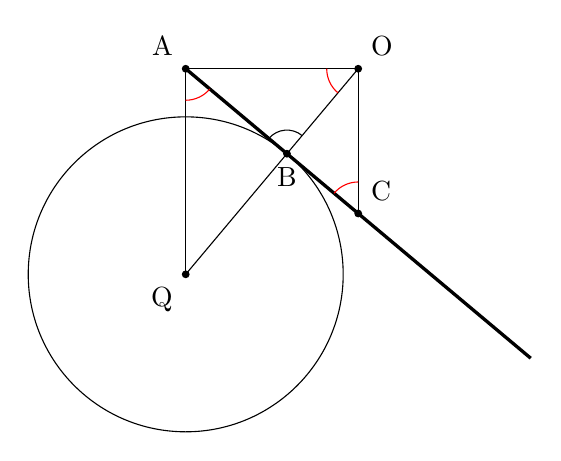
\begin{tikzpicture}
\usetikzlibrary{calc}
\def\angKatus{50};
\def\rKatus{2};
\coordinate (P1) at (0,{\rKatus/sin(\angKatus)});
\coordinate (P2) at ({\rKatus/sin(\angKatus)/tan(\angKatus)},{\rKatus/sin(\angKatus)});
\coordinate (P3) at ({\rKatus/sin(\angKatus)/tan(\angKatus)},{\rKatus/sin(\angKatus)-\rKatus/sin(\angKatus)/tan(\angKatus)/tan(\angKatus)});
%\fill (0,0) circle (0.05);
\node [label=below left:Q, fill=black, circle,inner sep=1pt] at (0,0){};
\draw (0,0) circle (\rKatus);
\node [label=above left:A, fill=black, circle,inner sep=1pt] at (P1){};
\node [label=above right:O, fill=black, circle,inner sep=1pt] at (P2){};
\node [label=above right:C, fill=black, circle,inner sep=1pt] at (P3){};
\node [label=below:B, fill=black, circle,inner sep=1pt] at (\angKatus:\rKatus){};
\draw [very thick](P1) -- (P3) -- ++($(P3)-(P1)$);
\draw (0,0) -- (P2);
\draw (0,0) -- (P1);
\draw (P1) -- (P2);
\draw (P3) -- (P2);
\draw [red](P1) ++ (-90:0.4) arc (-90:-90+\angKatus:0.4);
\draw [red](P3) ++ (90:0.4) arc (90:90+\angKatus:0.4);
\draw [red](P2) ++ (180:0.4) arc (180:180+\angKatus:0.4);
\draw (\angKatus:\rKatus) ++ (\angKatus:0.3) arc (\angKatus:90+\angKatus:0.3);
\end{tikzpicture}
\end{center}

Analyzing the stability we notice that if the “roof” would rotate as a whole then the center of mass moves along a circle and the only question would be if it is higher or lower than the cylinder’s axis $Q$; in the latter case the center of mass would be in the lowest location in the initial position and the system is stable. Therefore the stability condition is

$$|AQ|<|AC|\cos(\alpha/2).$$

If we replace this into the equation

$$|AQ|=|AB|/\cos(\alpha/2)=(L/2)\sin^2(\alpha/2)/\cos(\alpha/2)$$

and 

$$|AC|\cos(\alpha/2)=(L/2)\cos(\alpha/2),$$

then we get that $\sin^2(\alpha /2) < \cos ^2(\alpha /2)$. Because in the case of the roof $0<\frac{\alpha}{2}<90$ must apply then both sin and cos are positive and we can take a square root from both sides. We get the condition $\cos$ that applies when $\alpha<\pi/2$. Let us notice that the last condition can be presented in different ways using the relation between $R$, $L$ and $\alpha$.
\fi
}